%---------------------------------------------------------------------------
\svnidlong 
{$HeadURL: https://svn.fil.univ-lille1.fr/svn/sedoglav_PDC/trunk/Cours/05/05.tex $} 
{$LastChangedDate: 2010-10-01 12:32:44 +0200 (Fri, 01 Oct 2010) $} 
{$LastChangedRevision: 46 $} 
{$LastChangedBy: sedoglav $} 
\svnid{$Id: 05.tex 46 2010-10-01 10:32:44Z sedoglav $} 
%------------------------------------------------------------------------------
\begin{frame}[fragile]
    \section{Les pointeurs~: notions de base}
    Notion de pointeurs~:
    \begin{itemize}
    \item la m\'emoire physique est vue comme une suite finie
      d'octets~;
    \item un pointeur est une variable contenant l'adresse d'une autre variable~;
\begin{verbatim}
int i = 43 ; int *p_i ; p_i = &i ;
\end{verbatim}
    \item une valeur de type pointeur est une adresse m\'emoire~;
    \item un pointeur est donc un espace m\'emoire pouvant contenir
      une adresse~:
    \end{itemize}
    \par\bigskip
    \begin{footnotesize}
      \begin{center}
        \begin{tabular}{|l|c|c|c|c|c|c|c|c|c|c|c|}
          \hline
          label&\multicolumn{2}{c}{\ldots}\vline&\multicolumn{4}{l}{i}\vline
         &\multicolumn{4}{l}{p\_i}\vline&\ldots
          \\
          \hline
          adresse&0&\ldots         &x &x+1& x+2&x+3&x+4&x+5&x+6& x+7& \ldots
          \\    \hline
          octet&\multicolumn{2}{c}{\ldots}\vline&\multicolumn{4}{c}{43}\vline&\multicolumn{4}{c}{x}\vline&\ldots
          \\
          \hline
        \end{tabular}    
      \end{center}
    \end{footnotesize}
\end{frame}

%------------------------------------------------------------------------------
\begin{frame}[fragile]
\frametitle{D\'eclaration d'un pointeur}
\begin{itemize}
  \item pointeur~: caract\'eris\'e par le type de la variable point\'ee~;
  \item d\'eclaration~: {\it type\_point\'e} {\tt *}{\it identificateur\_pointeur} {\tt
      ;};
  \item {\it type\_point\'e}~: peut \^etre d'un type quelconque~;
  \item la classe d'allocation de la variable point\'ee peut \^etre
    tout sauf {\it register} i.e.\ la variable point\'ee peut \^etre
    externe, statique, automatique (voir cours correspondant)~;
  \item exemples~:

\begin{verbatim}
int foo ;                   .data                   
int *p_foo ;                 .globl foo   .size foo,4        
                      foo:   .long   44            
short int bar  ;             .globl p_foo .size p_foo,4    
short int *p_bar ;    p_foo: .long   foo           
                             .globl bar   .size bar,2        
foo=44 ; p_foo=&foo;  bar:   .value  44            
bar=44 ; p_bar=&bar;         .globl p_bar .size p_bar,4    
                      p_bar: .long   bar             
\end{verbatim}

\end{itemize}

\index{Pointeurs!d\'eclaration}
\index{Types!pointeurs}
\end{frame}
%------------------------------------------------------------------------------
\begin{frame}
    \section{Les op\'erateurs li\'es aux pointeurs}
    \frametitle{L'op\'erateur \&} 
    Cet op\'erateur retourne l'adresse d'un objet~: op\'erateur
    ``adresse de"
    \begin{itemize}
    \item il est unaire {\tt \&}~: adresse m\'emoire d'un objet~;
    \item il ne s'applique qu'\`a des objets en m\'emoire~: variables,
      \'el\'ements de tableaux, fonctions~;
    \item Exemple: {\tt int i, *p; p = \&i};
    \end{itemize}
    \par\bigskip
    
    On utilise une constante d\'enom\'ee ``pointeur nul''~: 
    \begin{center}
          {\tt \#define NULL 0}
    \end{center}
    et d\'efinie dans stddef.h (qui est inclus par le biais de
    stdio.h).  
    \par
    C'est la convention pour une adresse invalide
    (lorsqu'un pointeur n'est pas initialis\'e par exemple).
  \end{frame}
%------------------------------------------------------------------------------
\begin{frame}[fragile]
  \frametitle{L'op\'erateur {\tt *}} Il s'agit du
  d\'er\'ef\'erencement ou encore de l'op\'erateur d'indirection.
\begin{itemize}
\item c'est un op\'erateur unaire {\tt *} qui retourne la valeur de
  l'objet point\'e~;
\item il s'applique \`a un pointeur de mani\`ere pr\'efix\'ee~;
\item l'expression de retour est de m\^eme type que la valeur
  point\'ee~;
  \item il peut aussi appara\^\i{}tre en partie gauche d'affectation ({\it lvalue})~;
  \item Exemple~: \par
\begin{texttt}
  int i,j, *p = \&i ; \par
 *p = 4; j = *p + 1; 
\end{texttt}
\end{itemize}
\end{frame}
%------------------------------------------------------------------------------
\begin{frame}[fragile]
Exemple de d\'er\'ef\'erencement et d'utilisation d'un pointeur~:
\begin{verbatim}
/* avec les d\'efinitions      .text                     
   introduites dans les        .globl main                      
   transparents pr\'ec\'edents .type   main,@function   
*/                             main:                            
                                     ......                   
                               movl    p_bar, %eax      
int                            movswl  (%eax),%eax      
main                           addl    %eax, %eax       
(void)                         movw    %ax, bar         
{                              movl    p_foo, %edx      
   bar = *p_bar * 2 ;          movl    p_foo, %eax      
   *p_foo += 4 ;               movl    (%eax), %eax     
   return 0 ;                  addl    $4, %eax         
}                              movl    %eax, (%edx)     
                                  ......                   
\end{verbatim}
\end{frame}
%------------------------------------------------------------------------------
\begin{frame}[fragile]
  \frametitle{Attention}
  Les instructions~:
\begin{verbatim}
int foo ;
int *p_foo = &foo ;
\end{verbatim}
  ne sont pas \'equivalentes aux instructions~:
\begin{verbatim}
int foo ;
int *p_foo ;
*p_foo = &foo ;
\end{verbatim}
  \par\bigskip
  Il ne faut savoir sur quoi pointent vos pointeurs~; les instructions~:
\begin{verbatim}
int *ptr  ;
*ptr = 0 ;
\end{verbatim}
  provoqueront probablement une erreur de segmentation car \verb+ptr+
  n'est pas initialis\'e (on ne sait pas sur quoi il pointe).
\end{frame}
%------------------------------------------------------------------------------
\begin{frame}[fragile]
    \frametitle{Pointeur de type void}
    Pointeur vers le type {\tt void}~:
    \begin{itemize}
    \item pointeur vers un type \textit{quelconque}~;
    \item le d\'er\'ef\'erencement ne s'y applique pas~;
    \item utiliser l'op\'erateur de conversion explicite de type.
    \end{itemize}
    \par\bigskip\bigskip
    Exemple~:
\begin{verbatim}
int foo ;

void * p_qlcq = &foo  ;

int 
main
(void)
{
        foo =  * (int *) p_qlcq ;
        /*  "foo = *p_qlcq ; " est impossible */
        return 0 ;
}
\end{verbatim}
\end{frame}
%------------------------------------------------------------------------------
\begin{frame}[fragile]
    \frametitle{Affectation \`a un pointeur}
    Les pointeurs peuvent s'utiliser en valeur gauche (affectation)
    \`a condition que~:
\begin{itemize}
\item les pointeurs soient de m\^eme type i.e.\ m\^eme type d'objet
  point\'e~;
  \item on affecte l'adresse d'une variable du type point\'e~;
  \item l'expression de retour est un pointeur sur le type point\'e.
  \end{itemize}
  Il est possible d'affecter une constante pointeur {\tt NULL}.
\begin{verbatim}
int  a, *p_a =&a ;
char b, *p_b =&b ;
char c, *p_c =&c ;

   *p_a = *p_b ; /* conversion implicite */
   p_b  = p_c  ; /*   valide             */
/* p_a  = p_b  ;     invalide            */
\end{verbatim}

  \index{Op\'erateurs!adresse de}
\index{Op\'erateurs!d'indirection}
\index{Pointeurs!adresse d'un objet}
\index{Pointeurs!d\'er\'ef\'erencement}
\index{\verb?&? (adresse de)}
\index{\verb?*? (d\'er\'ef\'erencement)}
\end{frame}
%------------------------------------------------------------------------------
\begin{frame}[fragile]
    \section{Arithm\'etique sur les pointeurs}
    Addition d'un pointeur et d'un entier~: 
\begin{itemize}
  \item si {\tt p} est un pointeur vers des objets de type {\tt T}~;
  \item et {\tt n} est un  entier~;
  \item alors {\tt p + n} est une expression
    \begin{itemize}
    \item de type pointeur vers des objets de type {\tt T},
    \item et de valeur l'adresse du {\tt n}{\it i\`eme} objet suivant
      celui point\'e par {\tt p}~;
    \end{itemize}
  \item l'addition prend en compte la taille de l'objet.
\end{itemize}
\begin{verbatim}
int foo = 20 ;              .data                    
int *p_foo = &foo ;         .globl foo   .size   foo,4       
                      foo:  .long   20                  
int                         .globl p_foo .size   p_foo,4     
main                p_foo:  .long   foo     
(void)                      .text                    
{                           .globl main                      
  p_foo += 3 ;       main:   .........                
  return 0 ;                 addl    $12, p_foo       
}                           .........                
\end{verbatim}
\end{frame}
%------------------------------------------------------------------------------
\begin{frame}
  \frametitle{Sp\'ecificit\'e du type void * --- Soustraction}
  On ne peut faire de l'arithm\'etique de pointeurs de type void.
  \par\bigskip
 Soustraction d'un pointeur et d'un entier (identique \`a l'addition)~:
\begin{itemize}
\item la valeur \'etant l'adresse du {\tt n}{\it i\`eme} objet
  pr\'ec\'edent celui point\'e par~{\tt p}.
\end{itemize}
\index{Arithm\'etique!sur les pointeurs}
\index{Pointeurs!addition avec un entier}
\index{Pointeurs!affectation}
\par\bigskip
 Diff\'erence de pointeurs:
\begin{itemize}
\item si {\tt p} et {\tt q} sont des pointeurs de m\^eme type~;
  \item alors {\tt p - q} est une expression~:
    \begin{itemize}
    \item  de type entier,
      \item dont la valeur est le nombre d'objets situ\'es entre {\tt
          p} et {\tt q} inclus.
    \end{itemize}
\end{itemize}
\end{frame}
%------------------------------------------------------------------------------
\begin{frame}[fragile]
  \frametitle{Autres op\'erations}
 Comparaison de pointeurs~:
\begin{itemize}
  \item si {\tt p} et {\tt q} sont des  pointeurs de m\^eme type~;
  \item tous les op\'erateurs de comparaison sont utilisables~;
  \item {\tt p == q}~: m\^eme objet point\'e (adresse identique)~;
  \item \verb?p < q?~: {\tt p} pointe un objet pr\'ec\'edent celui
    point\'e par {\tt q}~;
  \item comparaison \`a {\tt NULL} possible.
\end{itemize}
 Calcul sur les pointeurs coh\'erent~:
\begin{itemize}
  \item prend en compte la taille des objets point\'es~;
  \item {\tt char *p; p=p+1;}~: fait ``avancer" {\tt p} de 1 octet~;
  \item {\tt int *p; p=p+1;}~: fait ``avancer" {\tt p} de 4 octets~;
  \item arithm\'etique bas\'ee sur la taille des objets point\'es ({\tt sizeof}).
\end{itemize}
 Tout autre calcul sur les pointeurs est {\em illicite}.
\index{Arithm\'etique!sur les pointeurs}
\index{Pointeurs!diff\'erence}
\index{Pointeurs!comparaison}

\end{frame}
%------------------------------------------------------------------------------
\begin{frame}
    \section{Pointeurs et passage de param\`etres par adresse}
    Lors de l'appel de fonction, le passage de param\`etres est par valeur~: \\
    \begin{center}
      \textbf{donc, pas d'effet de bord possible sur le param\`etre dans l'appelante.}
    \end{center}
    \par\smallskip
 Les pointeurs permettent un effet lat\'eral~: c'est le passage par adresse.
    \begin{center}
      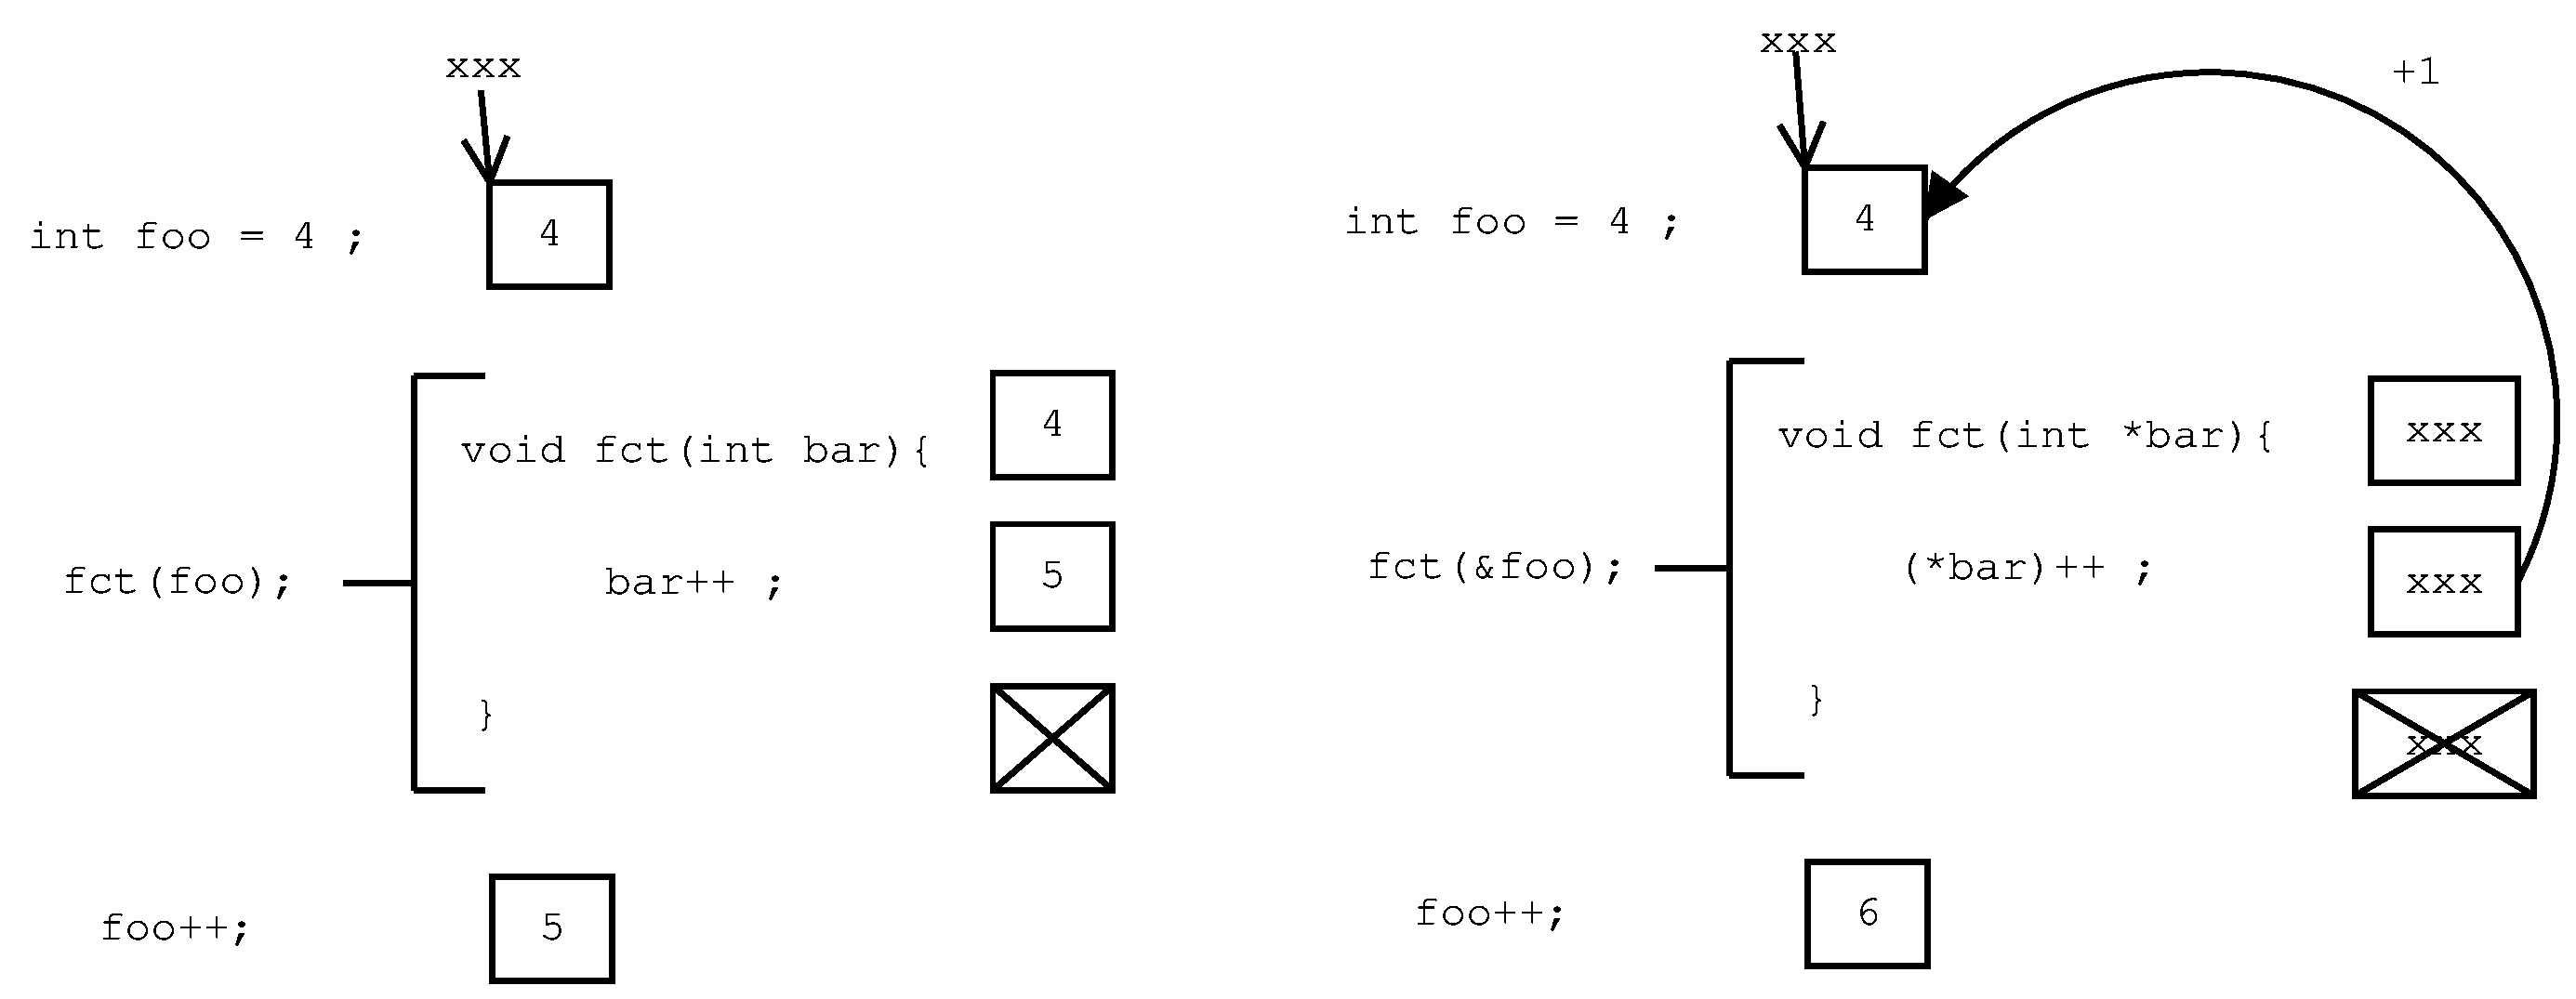
\includegraphics[scale=.22]{pointfunc}
    \end{center}
    \index{Pointeurs!et passage de param\`etres}
    \index{Passage de param\`etres!pointeurs}
\end{frame}
%------------------------------------------------------------------------------
\begin{frame}
  \section{Pointeurs et tableaux}
  Dans un langage "classique''~: apr\`es la d\'eclaration d'un tableau
  {\tt t}:
  \begin{itemize}
  \item {\tt t} est une variable~;
  \item {\tt t} est de type tableau de {\em quelque chose}~;
  \item {\tt t} d\'esigne le tableau en son entier.
  \end{itemize}
 En C~: 
\begin{itemize}
  \item {\tt t} {\bf n'est pas} une variable~;
  \item {\tt t} {\bf n'est pas} de type tableau de {\em quelque chose}~;
  \item {\tt t} {\bf ne d\'esigne pas} le tableau en son entier.
\end{itemize}
Ainsi, si on a {\tt int t[10];}~:
\begin{itemize}
  \item {\tt t} est une {\bf constante}~;
  \item {\tt t} est du type {\bf pointeur vers {\tt int}}~;
  \item valeur de {\tt t}~: adresse du premier \'el\'ement du tableau~;
    \begin{center}
        Si~{\tt t} est un tableau, alors {\tt t} $\equiv$ {\tt \&t[0]}.
    \end{center}
\end{itemize}
\index{Pointeurs!et tableaux}
\end{frame}
%------------------------------------------------------------------------------
\begin{frame}[fragile]
    \frametitle{Pointeurs et tableaux partagent abusivement des op\'erateurs}
    Il y a \'equivalence de notation~:
    \begin{center}
        Si {\tt t} est un tableau,  {\tt t[i]} $\equiv$ {\tt *(t
        + i)}
    \end{center}
\begin{itemize}
  \item un op\'erateur d'indexation est inutile dans le langage~;
  \item mais l'indexation est tout de m\^eme applicable \`a des variables de type
    pointeur~;
\end{itemize}
\begin{verbatim}
int tab[2] = { 1, 2 } ;              .data                 
                             tab:    .long   1,2
int *p = tab ;                 p:    .long   tab               
                                     .text                 
int                         main:   .....                  
main                                 movl    tab, %eax     
(void)                               movl    %eax, tab+4   
{                                    movl    p, %edx       
 *(tab+1) = *tab ;                   addl    $4, %edx      
  p[1] = p[0] ;                      movl    p, %eax       
  return 0 ;                         movl    (%eax), %eax  
}                                    movl    %eax, (%edx)  
\end{verbatim}
\end{frame}
%------------------------------------------------------------------------------
\begin{frame}[fragile]
    \frametitle{Passage de tableaux en param\`etre}
En cons\'equence des similitudes entre pointeurs et tableaux~: 
\begin{itemize}
  \item un param\`etre tableau est l'adresse du premier \'el\'ement~;
  \item c'est une {\em variable} locale \`a la fonction~: donc copie de 
    l'adresse~!!!! 
    \par
    \begin{bf}
      Le passage de param\`etre est syst\'ematiquement par adresse
      i.e.\ le tableau est modifi\'e~!!!
    \end{bf}
  \item deux syntaxes sont possibles~:
\begin{itemize}
\item par pointeur~:
{\normalsize
\begin{verbatim}
   void inc_tab(int *tableau, int size) {
     register int i;
     for (i = 0; i < size; i = i + 1;) 
       *(tableau + i) = *(tableau + i) + 1;
   }
\end{verbatim}
}
\item par tableau~:
{\normalsize
\begin{verbatim}
   void inc_tab(int tableau[], int size) {
     register int i;
     for (i = 0; i < size; i = i + 1;) 
       tableau[i] = tableau[i] + 1;
   }
\end{verbatim}
}
\end{itemize}
\end{itemize}

\index{Op\'erateurs!indexation d'un tableau}
\index{Pointeurs!et tableaux}
\index{Tableaux!pass\'es en param\`etre}

\end{frame}
%------------------------------------------------------------------------------
\begin{frame}[fragile]
  \frametitle{Pointeur et tableau multidimensionel (I)}%

\begin{verbatim}
                                         .globl tab .data            
char tab[3][4] = {"123","456","789"} ; tab:    .string "123"       
char *foo=NULL;                           .string "456"       
char bar=0 ;                              .string "789"       
int main(void){                           .globl foo                  
        foo = *(tab+1) ;               foo:    .long 0           
        bar = *(*(tab+2)) ;            .globl bar                  
        bar = foo[2] ;                 bar:    .byte 0           
        return 0 ;                        .text               
}                                      .globl main                 
                                       main:  .........
/* la syntaxe des pointeurs              movl $tab+4, foo 
   s'applique aux tableaux               movb tab+8, %al  
   et celles des tableaux                movb %al, bar    
   aux pointeurs bien qu'il ne           movl foo, %eax   
   s'agissent  pas exactement            addl $2, %eax    
   des m\^emes types d'objet */          movb (%eax), %al 
                                         movb %al, bar    
                                           ............
\end{verbatim}
\end{frame}
%------------------------------------------------------------------------------
\begin{frame}[fragile]
  \frametitle{Pointeur et tableau multidimensionel (II)}%
  Les pointeurs permettent un codage des tableaux multidimensionnels
  par un ``arbre''~:
\begin{verbatim}
#include <stdio.h>
char tab[3][4] = {"123","456","789"} ;

char *foo[3] = {NULL,NULL,NULL} ; /* ce sera char **foo ; */
                            /* lorsque nous saurons faire */          
int                         /* de l'allocation dynamique  */
main                        /* (prochain cours).          */      
(void)
{ 
     foo[0] = tab[0] ;     
     foo[1] = tab[1] ;     
     foo[2] = tab[2] ;                
     return (int) foo[1][1] ;                    
}                                       
\end{verbatim}
\end{frame}
%------------------------------------------------------------------------------
\begin{frame}[fragile]
 \section{Pointeurs de structures et d'union}
 \frametitle{Pointeurs et types compos\'es}
 Pointeur sur une structure~: usage de l'op\'erateur de s\'election \verb?->? 
 \par\smallskip
 En utilisant un exemple du cours pr\'ec\'edent~:
\begin{verbatim}
   struct adresse {  
     int num;        
     char rue[40];   
     long int code;  
     char ville[20]; 
   };                

   struct adresse var, *ptr = &var; 
  
   ptr->num=39; (*ptr).code = 59000 ;
   ptr->rue[0]=N ; (*ptr).rue[1] = i;
\end{verbatim}
\par
\begin{tabular}{lll}
  acc\`es~: & {\it (*pointeur\_union)}{\tt .}{\it membre} & ou \\
&  {\it pointeur\_union}\verb?->?{\it membre} 
 \end{tabular}
\end{frame}
%------------------------------------------------------------------------------
\begin{frame}[fragile]
\frametitle{On peut maintenant jouer avec les pointeurs\ldots}
\begin{verbatim}
enum bool_m {FALSE,TRUE} ;

enum bool_m *p_bool_v, bool_v ;

int 
main
(void) 
{
       bool_v   = TRUE    ;
       p_bool_v = &bool_v ;
       return *p_bool_v   ;
}
\end{verbatim}
\hfill tout en ayant une id\'ee claire de ce qui se passe en m\'emoire.  
\par
\hfill (au besoin, gdb peut nous aider).
\end{frame}
\end{document}


\begin{frame}

\section{Allocation dynamique}

 Fonction d'allocation dynamique de m\'emoire
\begin{itemize}
  \item fonction {\tt malloc} de la librairie standard;
  \item r\'eserve un espace m\'emoire dans le tas du processus;
\begin{tabular}[h]{|l|}
\hline
{\tt void *malloc(size\_t size)}\\
r\'eserve {\tt size} octets dans le tas et retourne un pointeur 
sur \\ la zone allou\'ee.\\
\hline
{\tt void free(void *ptr)}\\
lib\`ere une zone allou\'ee par un pr\'ec\'edent {\tt malloc}. {\tt ptr} doit
\\
obligatoirement \^etre un pointeur retourn\'e par un pr\'ec\'edent \\ {\tt
  malloc}.\\
\hline
\end{tabular}

\end{itemize}

 For\c{c}age de type: coercition (cast)
\begin{itemize}
\item force la conversion de type de la valeur d'un expression:\\
\hspace*{10mm} {\tt (}\hspace{3mm}{\it type}\hspace{3mm}{\tt
  )}\hspace{3mm}
{\it expression}
\item ne peut \^etre une valeur gauche;
\end{itemize}

 Taille d'un objet: op\'erateur {\tt sizeof}
\begin{tabular}[h]{|l|}
\hline
{\tt sizeof {\it expression}}\\
donne la taille en octets de son op\'erande {\tt expression}.\\
\hline
{\tt sizeof({\it identificateur\_de\_type})}\\
donne la taille en octets de tout objet de type \\
{\it identificateur\_de\_type}.\\
\hline
\end{tabular}

 Exemple
{\normalsize
\begin{verbatim}
   struct point {
      int x, y;
   };
   int n = 10;
   struct point *p_point;
   p_point = (struct point *)malloc(sizeof(struct point) * n);
\end{verbatim}
}

\index{Allocation dynamique}
\index{\verb?malloc?}
\index{\verb?free?}
\index{Coercition (cast)}
\index{Forcage de type}
\index{Op\'erateur!taille d'un objet}
\index{\verb?sizeof?}

\end{frame}



\begin{frame} 

\section{Les pointeurs de fonctions}

 Fonction en C
\begin{itemize}
  \item objet de premi\`ere classe: directement manipulable;
  \item d\'eclarateur postfixe {\tt ()}: {\tt int sqr(int x);}
  \item fonctionnement analogue \`a celui des tableaux:
    \begin{tabular}[h]{l|l}
D\'eclaration d'un tableau & D\'eclaration d'une fonction \\
de 5 entiers & enti\`ere \`a valeur enti\`ere \\
{\tt int ar[5];} & {\tt int sqr(int x);} \\
{\tt temp = ar[i]} & {\tt temp = sqr(i);} \\
d\'er\'ef\'erencement du pointeur & d\'er\'ef\'erencement du pointeur \\
d'entiers {\tt ar} et acc\`es & de fonction {\tt sqr} et appel \\
\`a son \'el\'ement {\tt i} & avec le param\`etre {\tt i}
    \end{tabular}
\newpage
  \item nom d'une fonction C = pointeur sur le d\'ebut du code
    correspondant \`a cette fonction. 

    {\bf
        Le nom d'une fonction en C a pour valeur un pointeur de
        fonction constant qui pointe sur elle m\^eme.
    }
\item Le nom d'une fonction est un pointeur de fonction {\tt constant}.
\end{itemize}
\par\medskip
 D\'eclaration d'une variable pointeur de fonction
\begin{itemize}
  \item identique au prototype en rajoutant une \verb?*?;
  \item d\'eclarer le type retourn\'e et le type des arguments;
  \item attention \`a la priorit\'e: op\'erateur droit $<<$ op\'erateur
    gauche.
\end{itemize}


 Exemple de d\'eclaration 
  \begin{itemize}
    \item {\tt int (*pf)(int, int);}: pointeur de fonction retournant
      un entier et prenant deux entiers en param\`etre;
  \item {\tt int *f(int, int)}: fonction retournant un pointeur
    sur un entier.
  \end{itemize}


\index{Types!pointeurs de fonction}
\index{Fonctions!pointeurs de}
\index{Pointeurs!de fonctions}
\end{frame}

\begin{frame}

\section{Les pointeurs de fonctions}


 Op\'erations sur les pointeurs de fonctions
\begin{itemize}
  \item assignation d'un pointeur de fonction \`a:
    \begin{itemize}
      \item un nom de fonction (pointeur constant);
      \item une variable de type pointeur de fonction;
      \item les types retourn\'es doivent \^etre {\em identiques};
    \end{itemize}
  \item Exemple d'assignation
{\normalsize
\begin{verbatim}
   int sqr(int x) {
     return x*x;
   }
   float fsqr(float x) {
     return x*x;
   }
   int (*pfint1)(int), (*pfint2)(int);

   pfint1 = sqr;
   pfint2 = pfint1;
   /* pfint2 = fsqr; ILLEGAL */
\end{verbatim}
}

\end{itemize}
\index{Pointeurs!de fonctions}
\end{frame}

\begin{frame} 

\section{Les pointeurs de fonctions}

\begin{itemize}
  \item appel de la fonction point\'ee: op\'erateur {\tt ()}
    \begin{itemize}
      \item d\'er\'ef\'erencer le pointeur de fonction;
      \item appeler la fonction point\'ee en donnant la liste des
        arguments entre {\tt ()};
      \item expression: type retourn\'e par la fonction;
      \item d\'er\'ef\'erencement facultatif en C-ANSI; 
    \end{itemize}
  \item Exemple d'appel
{\normalsize
\begin{verbatim}
   /* Avec les m\^emes d\'eclarations */
   int i;
  
   i = sqr(12);
   i = (*pfint1)(12);
   i = pfint1(12); /* C-ANSI */
\end{verbatim}
}
\end{itemize}
\newpage
 Exemples d'utilisation des pointeurs de fonction
\begin{itemize}
  \item Calcul de l'int\'egrale d'une fonction quelconque
{\normalsize
\begin{verbatim}
   int sqr3(int x) {
      return sqr(x) * x;
   }

   int integrale(int (*f)(int), int low, int high) {
     int i, aire = 0;
     for (i = low; i < high; i++) aire += (*f)(i);
     return aire;
   }

   void main(void) {
     printf("Aire de sqr sur [1, 10]: %d\n", integrale(sqr, 1, 10));
     printf("Aire de sqr3 sur [1, 10]: %d\n", integrale(sqr3, 1, 10));
   }
\end{verbatim}
}
\end{itemize}
\index{Pointeurs!de fonctions}
\index{Fonctions!appel par pointeur}
\end{frame}

\begin{frame}
    \section{Les pointeurs de fonctions}

    \begin{itemize}
      \item Menu de fonctions 
{\normalsize
\begin{verbatim}
   struct COMMANDE {
      char *nom ;
      void (*fun) (char *) ;
   } MENU [] = {
      {"ls", ls},
      {"cd", cd},
      {"more", more},
      {"cat",  cat},
      {0, }
     } ;
void executer (char *commande, char *argument)
{
   struct COMMANDE *p = MENU ;
   while (p->nom && strcmp (p->nom, commande)) p++ ;
   if (p->nom) {
      (*p->fun) (argument) ;
   } else fprintf (stderr, "%s : commande inconnue\n", commande) ;
}
\end{verbatim}
}
     \item Fonction quicksort de la librairie standard
{\normalsize
\begin{verbatim}
   extern void qsort(void *base, size_t nmemb, size_t size,
                     int (*compar)(const void *, const void *));
   typedef struct {
     char *nom;
     int note;
   } Etudiant;
   int inferieur(const Etudiant *p1, const Etudiant *p2) {
     if (p1->note < p2->note)
       return -1;
     else
       if (p1->note == p2->note)
         return(strcmp(p1->nom, p2->nom));
       else
         return 1;
   }
   Etudiant t[250];
   qsort(t, 250, sizeof(Etudiant), inferieur);
\end{verbatim}
}
    \end{itemize}

\index{\verb?qsort?}

\end{frame}

\begin{frame}
    \section{Les d\'eclarations complexes}

 {\tt int *(*(*x)())[5];}: 
\begin{itemize}
  \item {\tt (*x)}: x est un pointeur\ldots
  \item {\tt (*x)()}: de fonction qui retourne\ldots
  \item {\tt (*(*x)())}: un pointeur sur\ldots
  \item {\tt (*(*x)())[5]}: un tableau de 5\ldots
  \item {\tt int *(*(*x)())[5];}: pointeurs d'entiers;
\end{itemize}

 Probl\`eme des d\'eclarations complexes
\begin{itemize}
  \item op\'erateur pointeur \verb?*?: op\'erateur pr\'efixe;
  \item op\'erateurs tableau {\tt []} et fonction {\tt ()}: op\'erateurs
    postfixes;
  \item variable d'une d\'eclaration: noy\'ee dans des op\'erateurs;  
\end{itemize}
\end{frame}
%------------------------------------------------------------------------------
\begin{frame}
  M\'ethode
\begin{itemize}
  \item partir du nom de variable (ou de type);
  \item construire le type de l'int\'erieur vers l'ext\'erieur;
  \item appliquer les r\`egles suivantes:
    \begin{itemize}
      \item les op\'erateurs {\tt []} et {\tt ()} ont une plus grande
        priorit\'e que l'op\'erateur \verb?*?;

      \item les op\'erateurs {\tt []} et {\tt ()} se groupent de gauche
        \`a droite, alors que les op\'erateurs \verb?*? se groupent de
        droite \`a gauche; 
    \end{itemize}
\end{itemize}

 {\tt struct s (*(*(*x)[])())[];}

\index{D\'eclaration!complexe}

\end{frame}

%------------------------------------------------------------------------------
% That's all folks

